\chapter{The Raw Data}
\label{chap:rawdata}

Before any model could be trained, the raw data had to be understood, cleaned, and in several
places, repaired by hand. This chapter describes what the recordings actually looked like on
arrival, what was missing from them, and the concrete decisions taken to turn 22 raw recordings
and one imperfect annotation workbook into the 21-recording, 93-seizure dataset that everything
else in this report is built on.

\section{What we actually started with}

The project began with 22 recordings. Each one is a pair of raw MATLAB files --- one holding the
signal, one holding a header of technician notes --- plus a single \texttt{Annotations.xlsx}
workbook shared across all 22, listing each patient's seizure times and free-text notes.

Every recording was sampled at 256~Hz. This was not written anywhere in a header field: it had
to be decoded from the structure of the raw sample blocks themselves, which are organized in
1-second chunks of exactly 256 samples each.

The full channel montage, where present, was 19 EEG channels in the standard 10--20 layout, plus
an SLI channel (a pulse marker used during light stimulation testing), an ECG channel, and, in
some recordings, two EMG channels. Channel order was \emph{not} consistent from one file to the
next, so every channel was matched by its name, never trusted to sit in the same column twice.

Three things that should have been documented were not, and each had to be recovered from the
data itself rather than assumed:

\begin{itemize}[leftmargin=1.4em]
  \item \textbf{Sampling rate.} Not in any header field; decoded from the 256-sample blocks.
  \item \textbf{Channel order.} Not consistent file to file; channels are matched by name only.
  \item \textbf{Amplitude units.} No \texttt{varUnits} field, no description field, on any
    signal. Amplitude is reported throughout this project as ``unit not confirmed,'' and is
    never labeled microvolts without proof.
\end{itemize}

\section{What we cut, and why}

\subsection{One recording dropped entirely}

Recording \texttt{200625A\_F} had two problems at once: it carried only 8 of the 19 EEG
channels --- the 8 that happen to be common to every one of the 22 recordings --- and it had
zero seizure annotations of any kind.

Missing annotations do not prove a recording is seizure-free; they could just as easily mean a
label was never entered. Labeling this recording as a seizure-free control, on no evidence
either way, would have fed the model a guess dressed up as a fact. It was dropped entirely
instead. This leaves 21 recordings, every one of them with the full 19-channel EEG montage ---
the number quoted everywhere else in this report.

\subsection{What feeds the model, and what never does}

Only the 19 EEG channels are ever used as model input. The other signals and fields collected
alongside them are kept, but strictly as an audit tool, applied only \emph{after} a model has
already made its decisions:

\begin{itemize}[leftmargin=1.4em]
  \item \textbf{SLI pulses} --- checked against false alarms, to see whether a false alarm lands
    on a stimulation pulse.
  \item \textbf{ECG and EMG} --- checked for muscle-artifact bursts (an EMG RMS spike) behind a
    false alarm.
  \item \textbf{HPN notes} (the technician's hyperpnea markers, a seizure-provocation technique)
    --- checked for false alarms that coincide with a provocation period.
  \item \textbf{Sex, age, seizure count, seizure type, and the undocumented
    \texttt{Intercrit} markers} --- kept as separate patient metadata, never mixed into the
    training table.
\end{itemize}

The distinction is deliberate: these extra channels and fields make a model's errors
explainable after the fact, without ever being allowed to quietly influence the decision itself.

\subsection{Two clocks that never agreed}

The signal and the annotation workbook each start their own internal clock at zero, but the raw
files never recorded an absolute wall-clock start time. Seizure times in the workbook, meanwhile,
are stored as clock times of day --- for example \texttt{10:35:06} --- not as seconds already
relative to the start of the recording.

The correct conversion is
\[
  \text{elapsed seconds} = \text{clock time of the annotation} - \text{recording start time},
\]
with a midnight rollover applied when a seizure's clock time wraps past 00:00. Two shortcuts
were considered and explicitly rejected: treating the workbook's time as if it were already
relative seconds, and anchoring everything on the time of the first seizure. Either one would
have quietly fabricated labels rather than recovered real ones.

\begin{figure}[H]
  \centering
  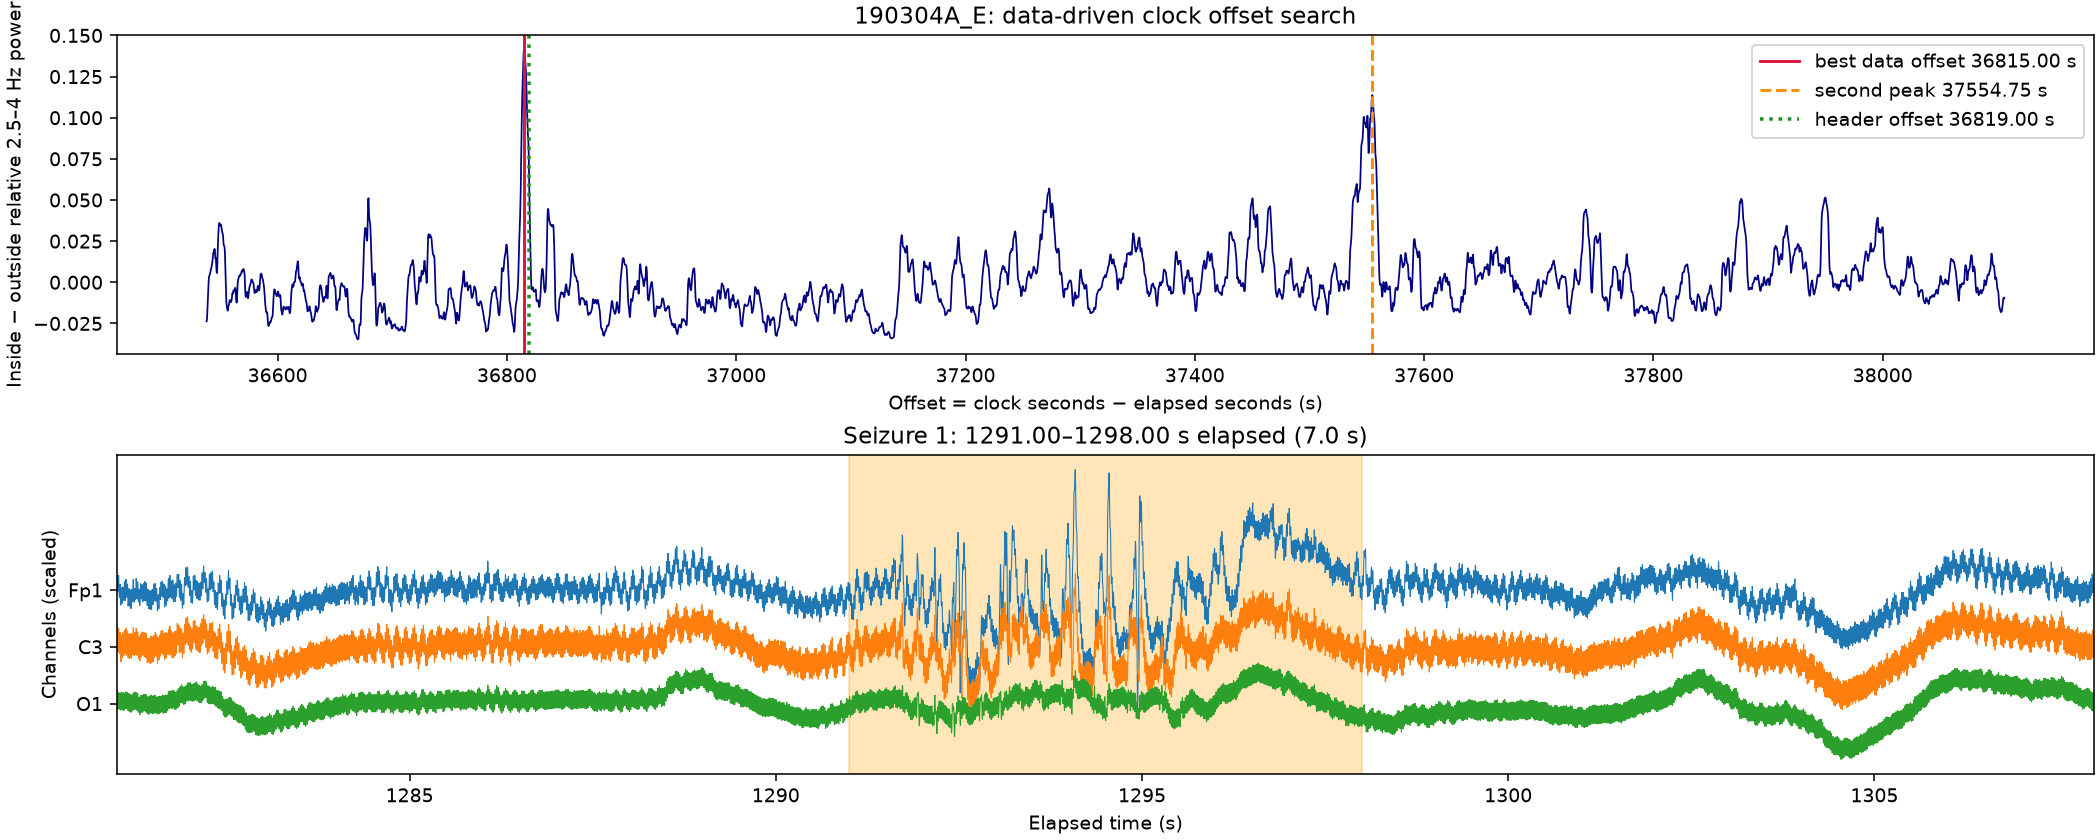
\includegraphics[width=0.85\linewidth]{offset_alignment/190304A_E_offset_alignment.png}
  \caption{Recovering the clock offset for recording \texttt{190304A\_E}: the technician's
    header markers are matched against the EEG signal itself to find the offset between the
    workbook's clock and the recording's internal clock.}
  \label{fig:offset-alignment-example}
\end{figure}

\subsection{When the labels disagreed, the signal decided}

Two recordings carried two conflicting candidate annotation rows each, with different proposed
seizure times for the same recording. Rather than pick a version by hand, each candidate
interval was scored against the real EEG: a seizure-likelihood score was computed inside the
candidate interval and outside it, and the candidate with the cleaner inside/outside separation
was kept.

\begin{table}[H]
  \centering
  \caption{Resolving the two conflicting annotation rows for \texttt{230406B\_A} by scoring each
    candidate against the real signal.}
  \label{tab:duplicate-rows}
  \begin{tabular}{lrrl}
    \toprule
    Candidate & Score & Inside/outside ratio & Decision \\
    \midrule
    Row 11 & 0.189 & 2.18 & Kept \\
    Row 19 & 0.173 & 2.09 & Dropped \\
    \bottomrule
  \end{tabular}
\end{table}

Recording \texttt{230515B\_G} was resolved the same way (row with ratio 4.08 kept over the row
with ratio 4.00). \texttt{210504B\_C}'s first seizure interval had a proposed end-time
correction that was validated the same way (score 0.306, ratio 2.61) and retained, and
\texttt{210427B\_C}'s official start time was validated likewise (score 0.306, ratio 2.70) and
included --- an important correction, since an earlier, now-archived version of the pipeline had
once excluded this recording for ``ambiguous alignment'' under a different, provisional
annotation set. That exclusion does not apply to the official dataset used in this report.

\begin{figure}[H]
  \centering
  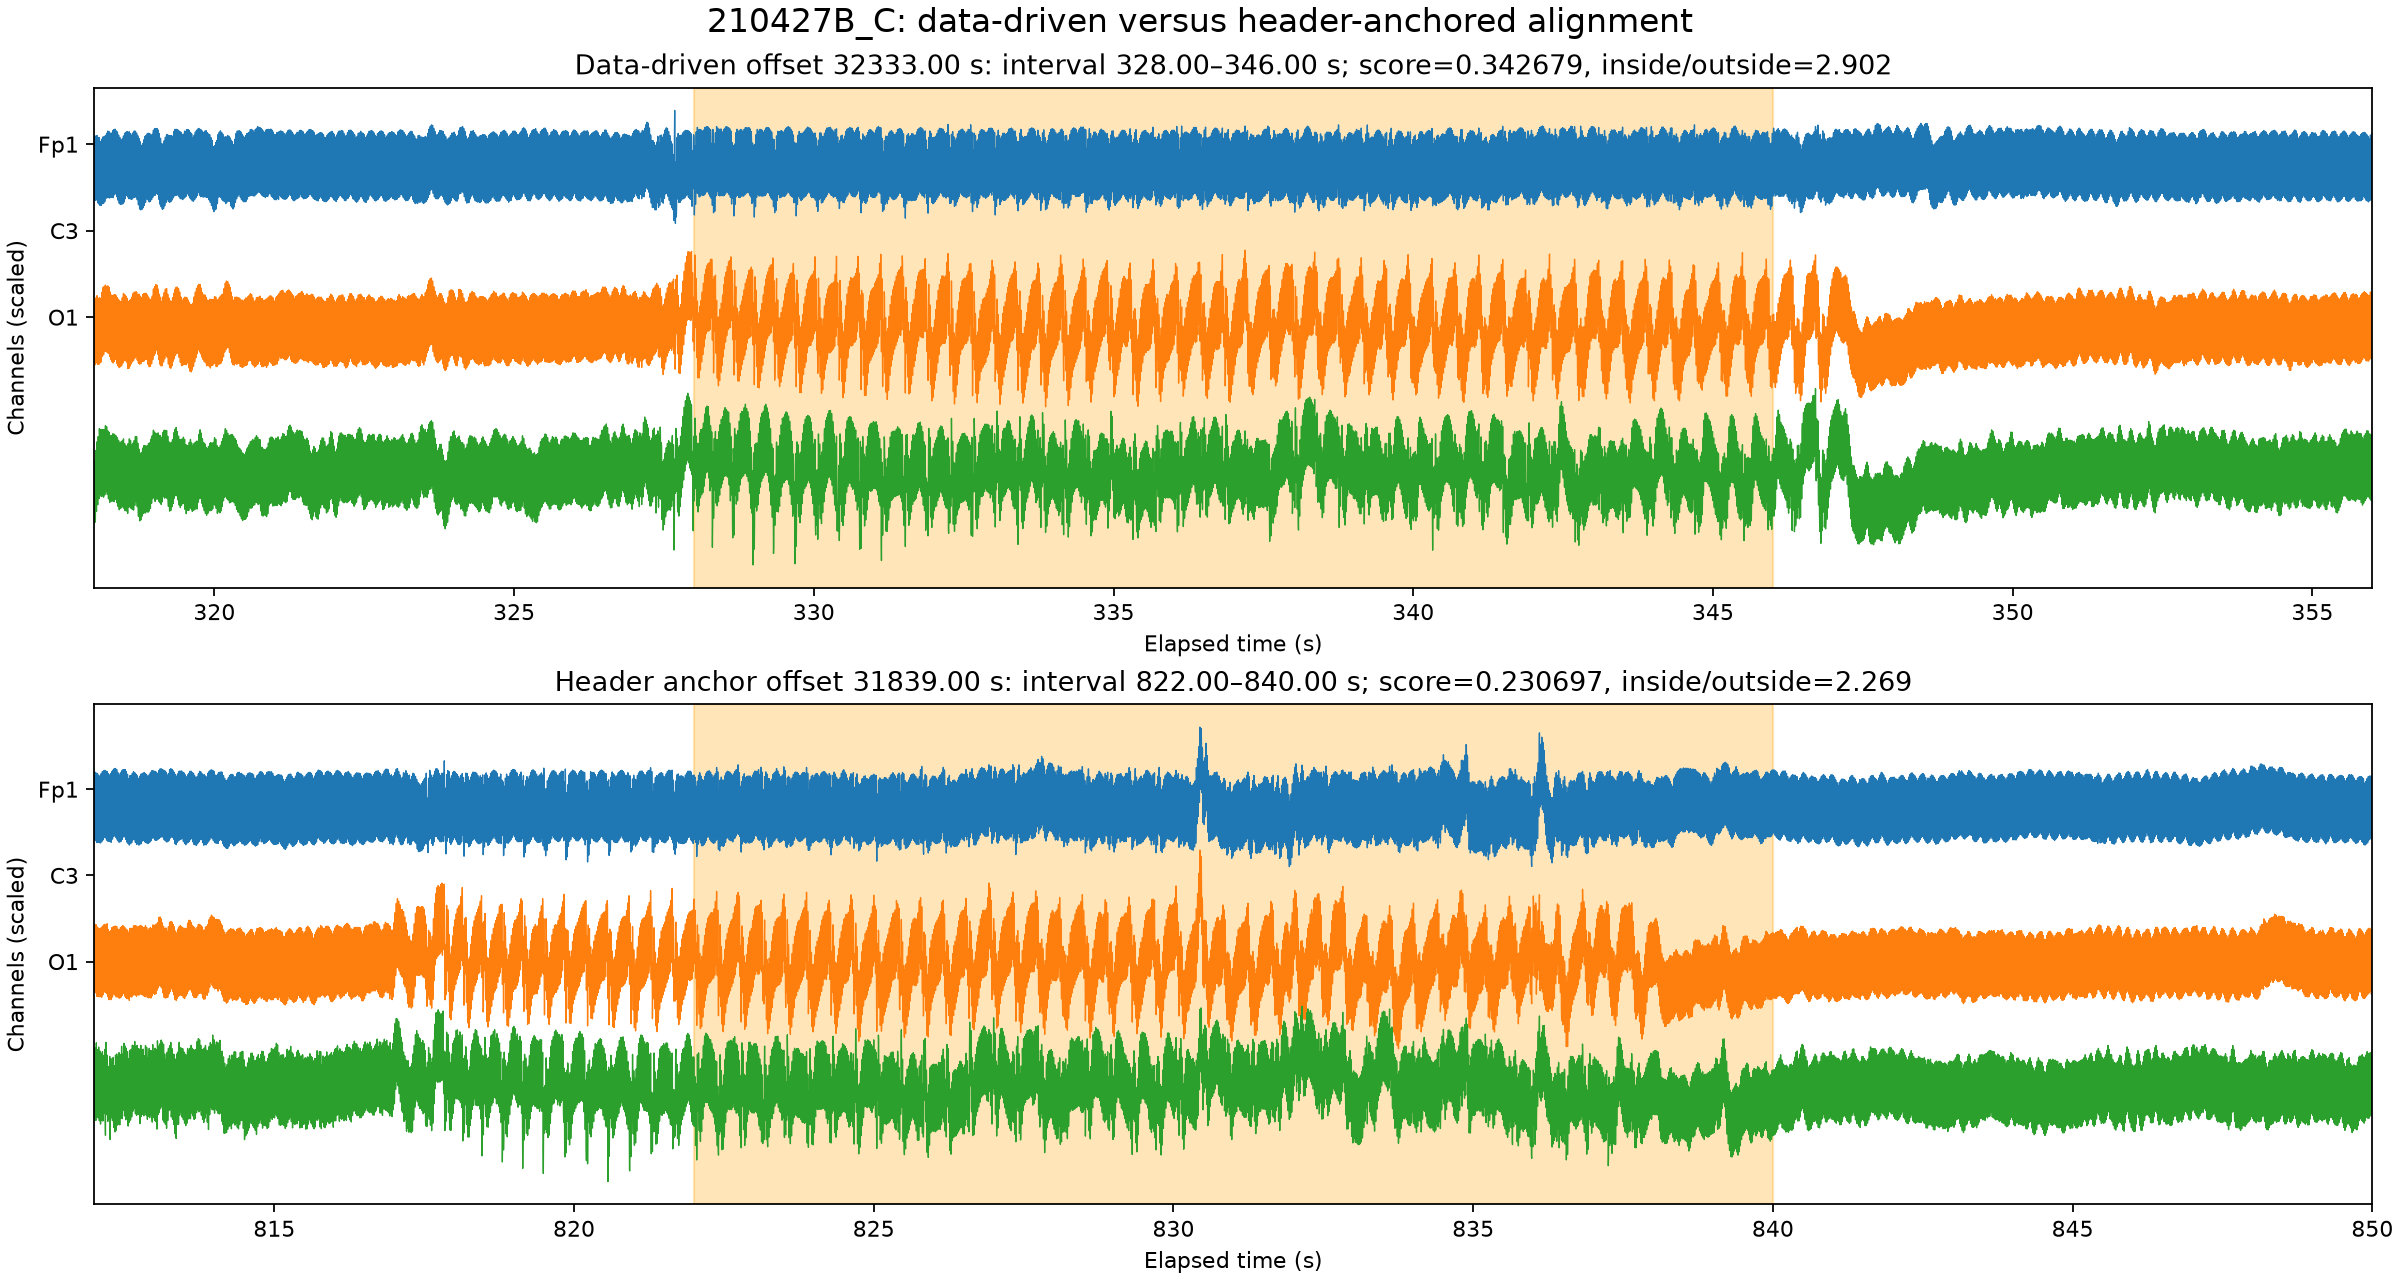
\includegraphics[width=0.85\linewidth]{offset_alignment/210427B_C_candidate_comparison.png}
  \caption{Comparing candidate seizure intervals for \texttt{210427B\_C} against the real
    signal, the method used to resolve every ambiguous or duplicate annotation row.}
  \label{fig:candidate-comparison}
\end{figure}

Two further recordings, \texttt{210204B\_C} and \texttt{210208B\_G}, are missing from the final,
corrected annotation workbook entirely. Both fall back to an earlier, provisional set of
intervals, rather than being invented or silently dropped.

\section{What survived the cleanup}

\begin{table}[H]
  \centering
  \caption{The dataset used throughout the rest of this report.}
  \label{tab:final-dataset}
  \begin{tabular}{lr}
    \toprule
    Recordings & 21 \\
    EEG channels per recording & 19 \\
    Confirmed, usable seizures & 93 \\
    Total recorded time & 8.73 hours (\texttt{models/registry.json}) \\
    \bottomrule
  \end{tabular}
\end{table}

From 22 recordings and one shared, imperfect workbook, this is the ground truth that every
later chapter is built on: the filter, the features, the twelve classical models, the deep
learning comparison, and the application all trace back to exactly these 21 recordings and
these 93 seizures.

\begin{summarybox}
The raw data arrived as 22 MATLAB recordings with no declared sampling rate, no declared
amplitude unit, inconsistent channel ordering, and seizure times with no absolute clock to
anchor them to. One recording was excluded for lacking both a full channel set and any
annotation; two recordings had genuinely conflicting annotation rows, resolved by scoring each
candidate against the real signal rather than by guessing; two more recordings, missing from the
final workbook, fell back to provisional intervals rather than being invented. The result is 21
recordings, 19 EEG channels each, 93 confirmed seizures --- the numbers used everywhere else in
this report.
\end{summarybox}
